\documentclass[portrait,final]{baposter}
%\documentclass[a4shrink,portrait,final]{baposter}
% Usa a4shrink for an a4 sized paper.

\tracingstats=2

\usepackage{times}
\usepackage{calc}
\usepackage{graphicx}
\usepackage{amsmath}
\usepackage{amssymb}
\usepackage{relsize}
\usepackage{multirow}
\usepackage{bm}

\usepackage{graphicx}
\usepackage{wrapfig}
\usepackage{multicol}

\usepackage{pgfbaselayers}
\pgfdeclarelayer{background}
\pgfdeclarelayer{foreground}
\pgfsetlayers{background,main,foreground}

\usepackage{helvet}
%\usepackage{bookman}
\usepackage{palatino}

\usepackage{url}
\usepackage{fancyvrb}

\newcommand{\captionfont}{\footnotesize}

\selectcolormodel{cmyk}

\graphicspath{{images/}}

%%%%%%%%%%%%%%%%%%%%%%%%%%%%%%%%%%%%%%%%%%%%%%%%%%%%%%%%%%%%%%%%%%%%%%%%%%%%%%%%
%%%% Some math symbols used in the text
%%%%%%%%%%%%%%%%%%%%%%%%%%%%%%%%%%%%%%%%%%%%%%%%%%%%%%%%%%%%%%%%%%%%%%%%%%%%%%%%
% Format 
\newcommand{\Matrix}[1]{\begin{bmatrix} #1 \end{bmatrix}}
\newcommand{\Vector}[1]{\Matrix{#1}}
\newcommand*{\SET}[1]  {\ensuremath{\mathcal{#1}}}
\newcommand*{\MAT}[1]  {\ensuremath{\mathbf{#1}}}
\newcommand*{\VEC}[1]  {\ensuremath{\bm{#1}}}
\newcommand*{\CONST}[1]{\ensuremath{\mathit{#1}}}
\newcommand*{\norm}[1]{\mathopen\| #1 \mathclose\|}% use instead of $\|x\|$
\newcommand*{\abs}[1]{\mathopen| #1 \mathclose|}% use instead of $\|x\|$
\newcommand*{\absLR}[1]{\left| #1 \right|}% use instead of $\|x\|$

\def\norm#1{\mathopen\| #1 \mathclose\|}% use instead of $\|x\|$
\newcommand{\normLR}[1]{\left\| #1 \right\|}% use instead of $\|x\|$

%%%%%%%%%%%%%%%%%%%%%%%%%%%%%%%%%%%%%%%%%%%%%%%%%%%%%%%%%%%%%%%%%%%%%%%%%%%%%%%%
% Multicol Settings
%%%%%%%%%%%%%%%%%%%%%%%%%%%%%%%%%%%%%%%%%%%%%%%%%%%%%%%%%%%%%%%%%%%%%%%%%%%%%%%%
\setlength{\columnsep}{0.7em}
\setlength{\columnseprule}{0mm}


%%%%%%%%%%%%%%%%%%%%%%%%%%%%%%%%%%%%%%%%%%%%%%%%%%%%%%%%%%%%%%%%%%%%%%%%%%%%%%%%
% Save space in lists. Use this after the opening of the list
%%%%%%%%%%%%%%%%%%%%%%%%%%%%%%%%%%%%%%%%%%%%%%%%%%%%%%%%%%%%%%%%%%%%%%%%%%%%%%%%
\newcommand{\compresslist}{%
\setlength{\itemsep}{1pt}%
\setlength{\parskip}{0pt}%
\setlength{\parsep}{0pt}%
}


%%%%%%%%%%%%%%%%%%%%%%%%%%%%%%%%%%%%%%%%%%%%%%%%%%%%%%%%%%%%%%%%%%%%%%%%%%%%%%
%%% Begin of Document
%%%%%%%%%%%%%%%%%%%%%%%%%%%%%%%%%%%%%%%%%%%%%%%%%%%%%%%%%%%%%%%%%%%%%%%%%%%%%%

\begin{document}

%%%%%%%%%%%%%%%%%%%%%%%%%%%%%%%%%%%%%%%%%%%%%%%%%%%%%%%%%%%%%%%%%%%%%%%%%%%%%%
%%% Here starts the poster
%%%---------------------------------------------------------------------------
%%% Format it to your taste with the options
%%%%%%%%%%%%%%%%%%%%%%%%%%%%%%%%%%%%%%%%%%%%%%%%%%%%%%%%%%%%%%%%%%%%%%%%%%%%%%
% Define some colors
\definecolor{silver}{cmyk}{0,0,0,0.3}
\definecolor{yellow}{cmyk}{0,0,0.9,0.0}
\definecolor{reddishyellow}{cmyk}{0,0.22,1.0,0.0}
\definecolor{black}{cmyk}{0,0,0.0,1.0}
\definecolor{darkYellow}{cmyk}{0,0,1.0,0.5}
\definecolor{darkSilver}{cmyk}{0,0,0,0.1}

\definecolor{lightyellow}{cmyk}{0,0,0.3,0.0}
\definecolor{lighteryellow}{cmyk}{0,0,0.1,0.0}
\definecolor{lighteryellow}{cmyk}{0,0,0.1,0.0}
\definecolor{lightestyellow}{cmyk}{0,0,0.05,0.0}

\definecolor{white}{cmyk}{0,0,0,0}
\definecolor{gray5}{cmyk}{0,0,0,0.05}
\definecolor{gray30}{cmyk}{0,0,0,0.3}
\definecolor{gray50}{cmyk}{0,0,0,0.5}
\definecolor{gray90}{cmyk}{0,0,0,0.9}

%%
\typeout{Poster Starts}
\background{
  \begin{tikzpicture}[remember picture,overlay]%
    \draw (current page.north west)+(-2em,2em) node[anchor=north west] {
\includegraphics[height=1.1\textheight]{silhouettes_background}};
  \end{tikzpicture}%
}

\newlength{\leftimgwidth}
\begin{poster}%
  % Poster Options
  {
  % Show grid to help with alignment
  grid=no,
  % Column spacing
  colspacing=1em,
  % Color style
  bgColorOne=white,
  bgColorTwo=white,
  borderColor=black,
  headerColorOne=gray50,
  headerColorTwo=gray90,
  headerFontColor=reddishyellow,
  boxColorOne=gray5,
  boxColorTwo=gray5,
  % Format of textbox
  textborder=none, %rectangle,
  textfont=\sf, %Sans Serif
 % Format of text header
  eyecatcher=no,
  headerborder=none,
  headerheight=0.08\textheight,
  headershape=rectangle,
  headershade=shade-tb,
  headerfont=\Large\textsf, %Sans Serif
  boxshade=none, %shade-tb,
%  background=shade-tb,
  background=none,
  linewidth=2pt
  }
 % Eye Catcher
  {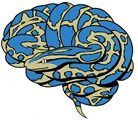
\includegraphics[width=1em]{nipylogo}} % No eye catcher for this poster. (eyecatcher=no above). If an eye catcher is present, the title is centered between eye-catcher and logo.
  % Title
  {\sf %Sans Serif
  %\bf% Serif
  Distributed Neuroimaging Analysis with Nipype and IPython\vspace{0.15em}}
  % Authors
  {\sf %Sans Serif
  % Serif
  Satrajit Ghosh$^1$, Brian Granger$^2$, Fernando Perez$^3$\\
  \small\sf$^1$MIT, Cambridge, MA $^2$California Polytechnic State
  University, San Luis Obispo, CA $^3$University of California,
  Berkeley, CA}


  % University logo
  % {% The makebox allows the title to flow into the logo, this is a hack because of the L shaped logo.
  %   \makebox[8em][r]{%
  %     \begin{minipage}{16em}
  %       \hfill
  %       %\includegraphics[height=2em]{msrlogo}
  %       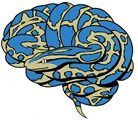
\includegraphics[height=7.0em]{nipylogo}
  %     \end{minipage}
  %   }
  % }

  \tikzstyle{light shaded}=[top color=baposterBGtwo!30!white,bottom color=baposterBGone!30!white,shading=axis,shading angle=30]

  % Width of left inset image
     \setlength{\leftimgwidth}{0.78em+8.0em}

%%%%%%%%%%%%%%%%%%%%%%%%%%%%%%%%%%%%%%%%%%%%%%%%%%%%%%%%%%%%%%%%%%%%%%%%%%%%%%
%%% Now define the boxes that make up the poster
%%%---------------------------------------------------------------------------
%%% Each box has a name and can be placed absolutely or relatively.
%%% The only inconvenience is that you can only specify a relative position 
%%% towards an already declared box. So if you have a box attached to the 
%%% bottom, one to the top and a third one which should be in between, you 
%%% have to specify the top and bottom boxes before you specify the middle 
%%% box.
%%%%%%%%%%%%%%%%%%%%%%%%%%%%%%%%%%%%%%%%%%%%%%%%%%%%%%%%%%%%%%%%%%%%%%%%%%%%%%
    %
    % A coloured circle useful as a bullet with an adjustably strong filling
   \newcommand{\colouredcircle}[1]{%
      \tikz{\useasboundingbox (-0.2em,-0.32em) rectangle(0.2em,0.32em); \draw[draw=black,fill=headerFontColor!80!black!#1!white,line width=0.03em] (0,0) circle(0.18em);}}
    \renewcommand{\labelitemi}{\colouredcircle{100}}
    \renewcommand{\labelitemii}{\colouredcircle{50}}

%%%%%%%%%%%%%%%%%%%%%%%%%%%%%%%%%%%%%%%%%%%%%%%%%%%%%%%%%%%%%%%%%%%%%%%%%%%%%%
  \headerbox{Introduction}{name=introduction,column=0,row=0}{
%%%%%%%%%%%%%%%%%%%%%%%%%%%%%%%%%%%%%%%%%%%%%%%%%%%%%%%%%%%%%%%%%%%%%%%%%%%%%%
    We present distributed execution of neuroimaging analysis pipelines
    that the open source Nipype \cite{ghos.python-based.09} project has
    developed by integrating with IPython's \cite{pere.ipython.07}
    parallel computing facilities. Today we face an explosion in the
    size and complexity of neuroimaging datasets, whose analysis
    requires not only sophisticated algorithms but computational
    infrastructure to support their use with ease, efficiency,
    reliability and reproducibility. 

    While existing analysis packages provide excellent tools, they often
    constrain users to specific workflows and environments. Furthermore,
    very few of the available neuroimaging tools take advantage of the
    growing number of parallel hardware configurations (multicore,
    clusters, clouds and supercomputers) or integration with
    neuroimaging databases. By using IPython's high-level facilities for
    distributed computing, Nipype can optimally execute any
    parallelizable analysis pipeline.  \vspace{0.3em} }

%%%%%%%%%%%%%%%%%%%%%%%%%%%%%%%%%%%%%%%%%%%%%%%%%%%%%%%%%%%%%%%%%%%%%%%%%%%%%%
  \headerbox{Features}{name=features,column=0,below=introduction}{
%%%%%%%%%%%%%%%%%%%%%%%%%%%%%%%%%%%%%%%%%%%%%%%%%%%%%%%%%%%%%%%%%%%%%%%%%%%%%%
    \begin{list}{\labelitemi}{\leftmargin=1em}
      \compresslist
      \item Parallel execution of workflows
      \item No additional coding for parallel execution
      \item Supports SPM, FSL, FreeSurfer
      \item Automatic load balancing across cluster
    \end{list}
  }

%%%%%%%%%%%%%%%%%%%%%%%%%%%%%%%%%%%%%%%%%%%%%%%%%%%%%%%%%%%%%%%%%%%%%%%%%%%%%%
  \headerbox{Nipype}{name=nipype,column=1,row=0}{
%%%%%%%%%%%%%%%%%%%%%%%%%%%%%%%%%%%%%%%%%%%%%%%%%%%%%%%%%%%%%%%%%%%%%%%%%%%%%%

    Current neuroimaging software offer users an incredible opportunity
    to analyze their data in different ways, with different underlying
    assumptions. However, this has resulted in a heterogeneous
    collection of specialized applications without transparent
    interoperability or a uniform operating interface.

    Nipype, an open-source, community-developed initiative under the
    umbrella of Nipy, is a Python project that solves these issues by
    providing a uniform interface to existing neuroimaging software and
    by facilitating interaction between these packages within a single
    workflow. 

    Nipype provides an environment that encourages interactive
    exploration of algorithms from different packages (e.g., SPM, FSL,
    FreeSurfer), eases the design of workflows within and between
    packages, and reduces the learning curve necessary to use different
    packages. 

    Nipype is creating a collaborative platform for
    neuroimaging software development in a high-level language and
    addressing limitations of existing pipeline systems. Nipype is
    accessible via NITRC (http://www.nitrc.org/projects/nipype/) and is
    written in Python, a free high-level language with extensive
    scientific computation capabilities that is accessible to both
    programmers and non-programmers.

 \vspace{0.5em}
  }

%%%%%%%%%%%%%%%%%%%%%%%%%%%%%%%%%%%%%%%%%%%%%%%%%%%%%%%%%%%%%%%%%%%%%%%%%%%%%%
  \headerbox{IPython}{name=ipython,column=2,row=0}{
%%%%%%%%%%%%%%%%%%%%%%%%%%%%%%%%%%%%%%%%%%%%%%%%%%%%%%%%%%%%%%%%%%%%%%%%%%%%%%
    IPython SUMMARY here.

    The goal of IPython is to create a comprehensive environment for
    interactive and exploratory computing. To support, this goal,
    IPython has two main components:

    \begin{itemize}
      \compresslist
      \item An enhanced interactive Python shell.
      \item An architecture for interactive parallel computing.  
    \end{itemize}
\vspace{0.5em}
  }

%%%%%%%%%%%%%%%%%%%%%%%%%%%%%%%%%%%%%%%%%%%%%%%%%%%%%%%%%%%%%%%%%%%%%%%%%%%%%%
  \headerbox{Funding}{name=funding,column=1,span=2,above=bottom}{
%%%%%%%%%%%%%%%%%%%%%%%%%%%%%%%%%%%%%%%%%%%%%%%%%%%%%%%%%%%%%%%%%%%%%%%%%%%%%%
    \smaller This project was supported by NIH grants NIBIB R03 EB008673
    (PI: Ghosh, Whitfield-Gabrieli), NIMH R01 MH081909 (PI: D'Esposito).
  }

%%%%%%%%%%%%%%%%%%%%%%%%%%%%%%%%%%%%%%%%%%%%%%%%%%%%%%%%%%%%%%%%%%%%%%%%%%%%%%
  \headerbox{Results}{name=results,column=1,span=2,below=nipype,above=funding}{
%%%%%%%%%%%%%%%%%%%%%%%%%%%%%%%%%%%%%%%%%%%%%%%%%%%%%%%%%%%%%%%%%%%%%%%%%%%%%%
  \begin{tikzpicture}[x=\linewidth,y=\linewidth]
    %\path [use as bounding box] (-0.5,-0.5) rectangle(2.5,1.7);
    \node{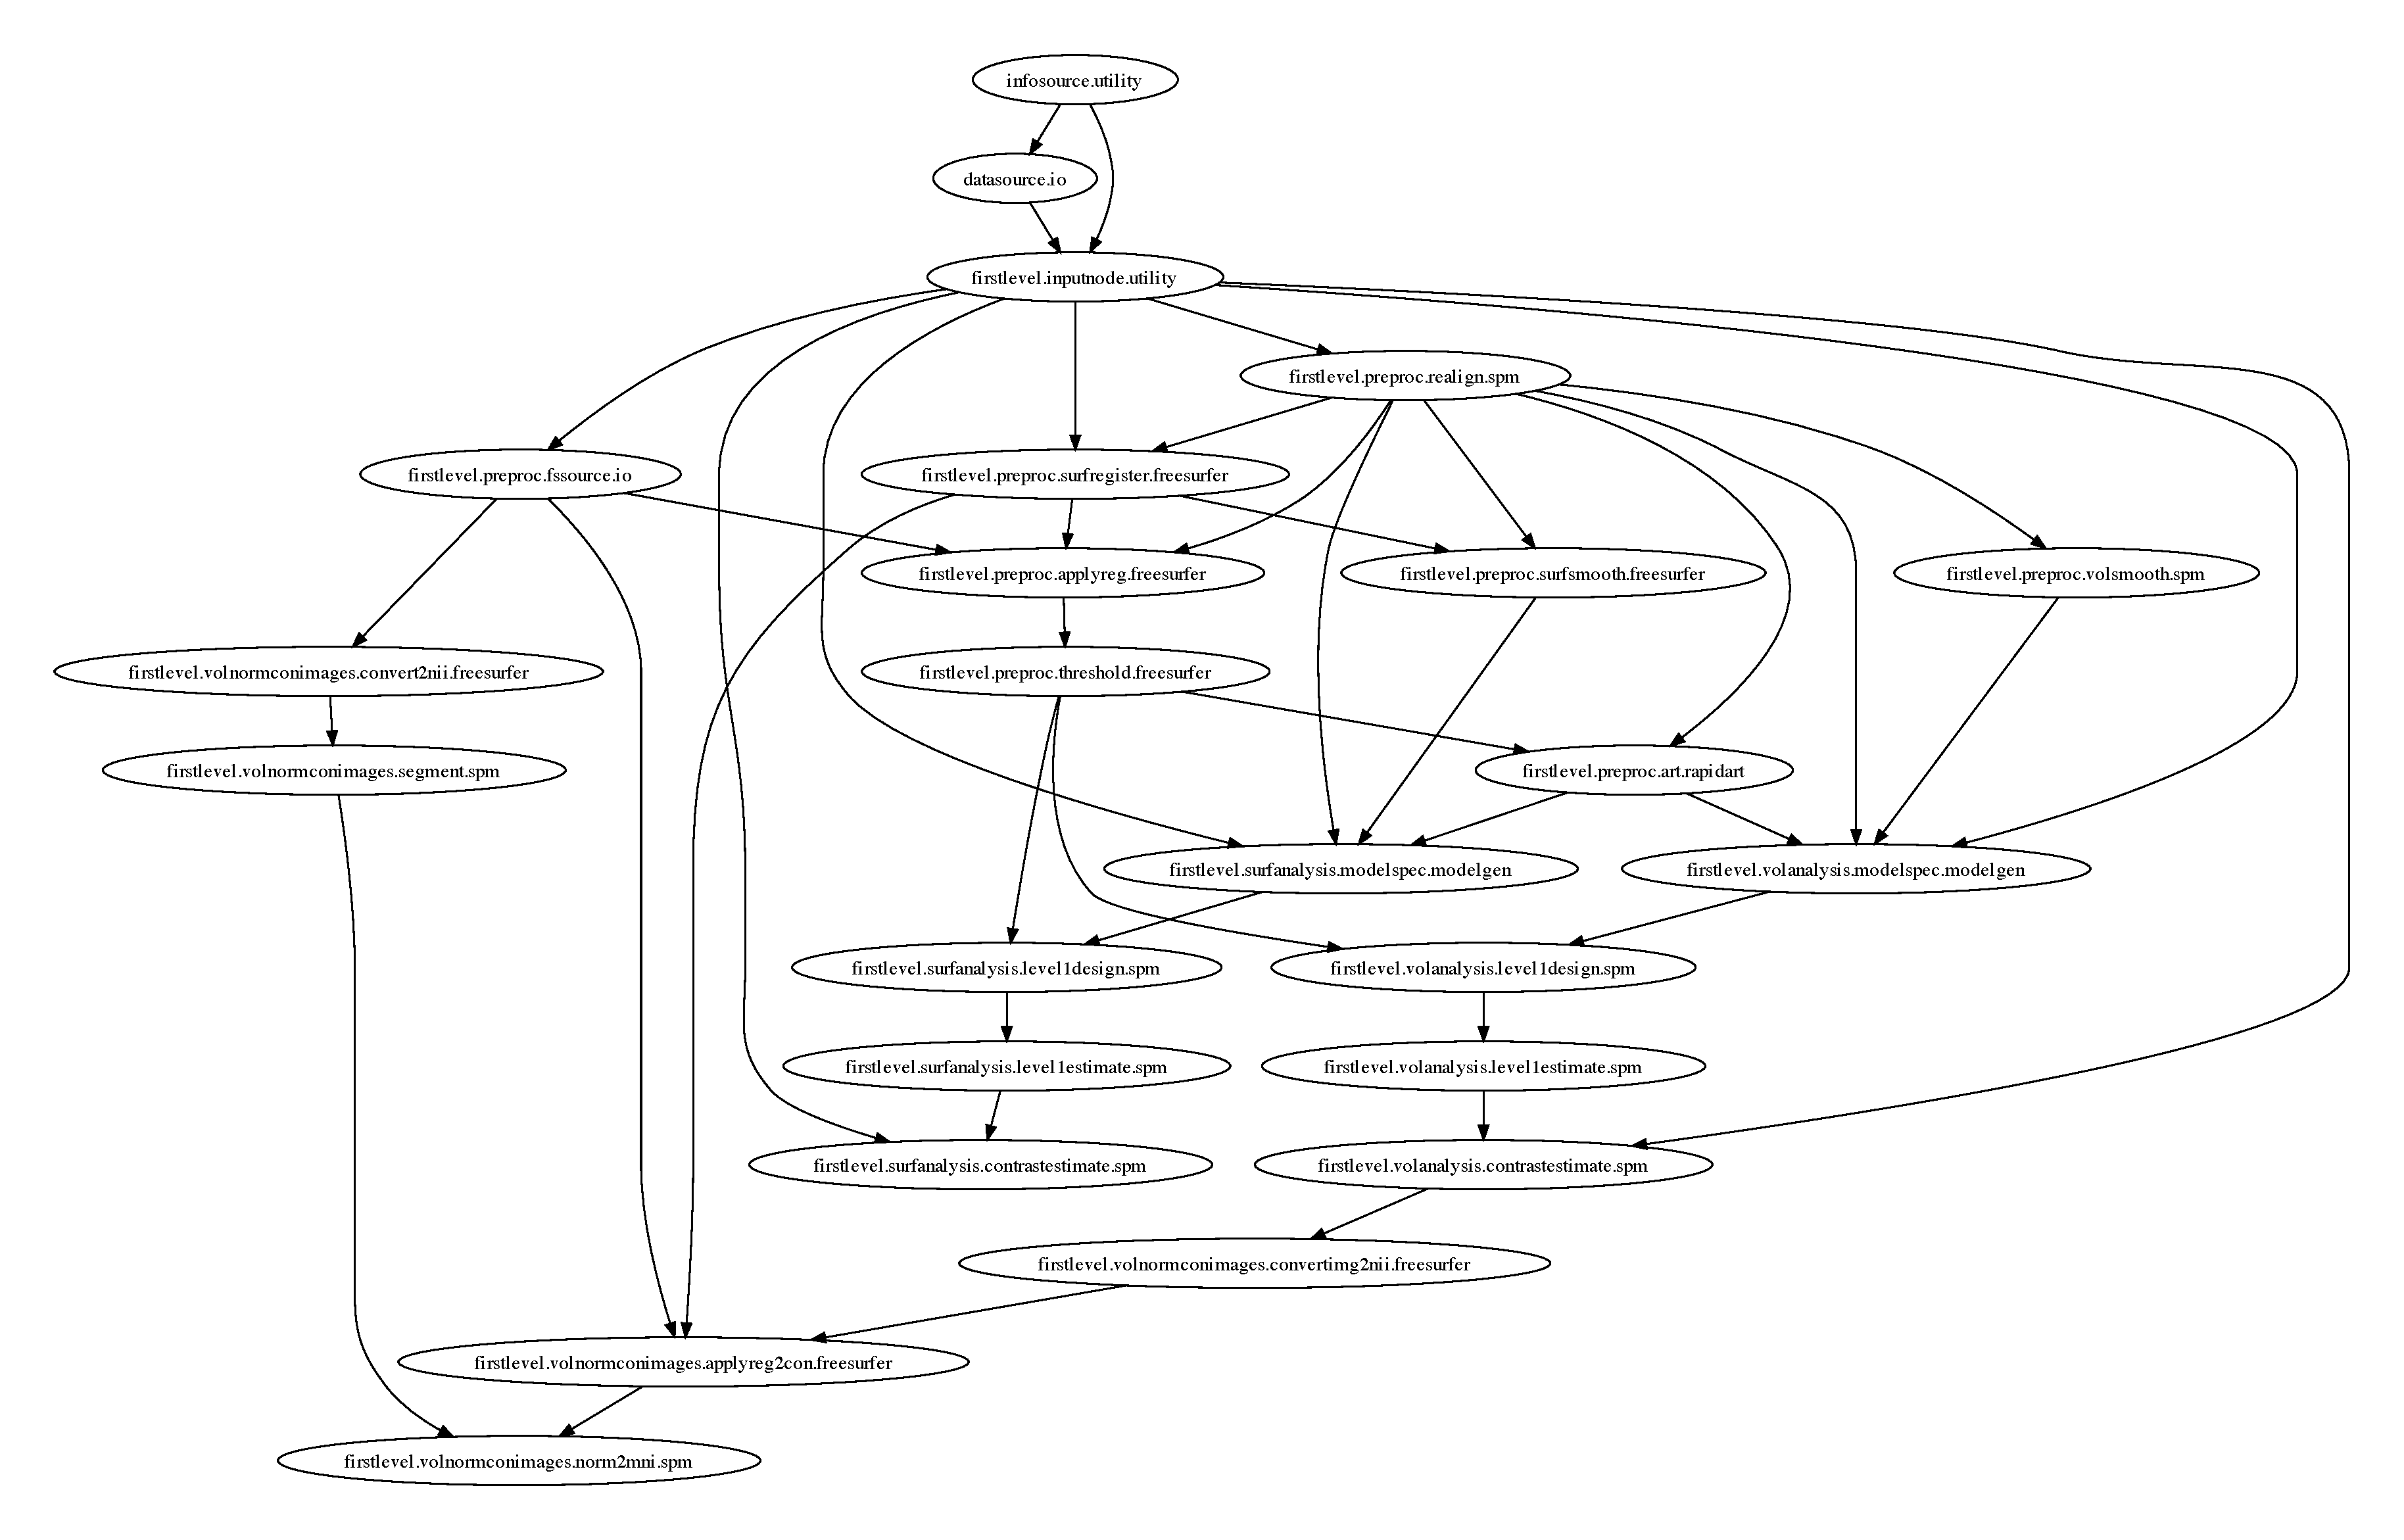
\includegraphics[width=\linewidth]{nipype_graph}};
 \end{tikzpicture}
      \begin{multicols}{2}
        Parallel execution was evaluated on two datasets. One comprising
        an SPM workflow and one comprising a comparative workflow. SATRA
        fill rest and timing results.\\
   \end{multicols}\vspace{-1em}
      \mbox{\hspace{0.3\linewidth}\rule{0.4\linewidth}{1pt}\hspace{0.3\linewidth}}\\
\vspace{0.5em}
  }

%%%%%%%%%%%%%%%%%%%%%%%%%%%%%%%%%%%%%%%%%%%%%%%%%%%%%%%%%%%%%%%%%%%%%%%%%%%%%%
  \headerbox{References}{name=references,column=0,above=bottom}{
%%%%%%%%%%%%%%%%%%%%%%%%%%%%%%%%%%%%%%%%%%%%%%%%%%%%%%%%%%%%%%%%%%%%%%%%%%%%%%
    \smaller
    \vspace{-0.4em}
    \bibliographystyle{ieee}
    \renewcommand{\section}[2]{\vskip 0.05em}
    \bibliography{poster}
 }

%%%%%%%%%%%%%%%%%%%%%%%%%%%%%%%%%%%%%%%%%%%%%%%%%%%%%%%%%%%%%%%%%%%%%%%%%%%%%%
  \headerbox{Conclusion}{name=conclusion,column=0,span=1,below=features,above=references}{
%%%%%%%%%%%%%%%%%%%%%%%%%%%%%%%%%%%%%%%%%%%%%%%%%%%%%%%%%%%%%%%%%%%%%%%%%%%%%%
    We have developed a practical integration of IPython's parallel and
    distributed computing capabilities into Nipype's pipeline execution
    machinery. This provides an easy to use system for parallelizing
    analysis tasks with minimal effort and without the requirement for
    explicit parallel programming. Currently, one can execute SPM, FSL
    and a variety of FreeSurfer functions in parallel using this system
    on variety of different distributed computing architectures as long
    as they share a common file-system and have all underlying tools
    installed. Future improvements will focus on moving the DAG
    scheduler to IPython itself for efficient load balancing,
    file-system independent execution, selective execution of nodes on
    compatible systems (e.g., run FSL and FreeSurfer nodes only on unix
    systems in a mixed operating system cluster), interfacing with cloud
    services and support of more neuroimaging analysis packages.  }

\end{poster}%
\end{document}
